\documentclass[12pt]{article}

\usepackage{url} % websites in bib
\usepackage{hyperref}
\usepackage[a4paper,left=1in,right=1in,top=1in,bottom=1in]{geometry} % margins
\usepackage{paralist} % compact enumerates

\usepackage{graphicx}
\usepackage{caption}
\usepackage{subcaption}

\begin{document}
	\title{K-Means clustering variants and improvements}
	\author{Stefan Sebastian, 242}
	\maketitle
	
	\begin{abstract}
		TODO make abstract
	\end{abstract}

	\newpage
	\tableofcontents
	\newpage
	
	\section{Introduction}
	\subsection{Motivation}
	In recent times there has been an explosive growth of data. This new, digital resource has become so important that a recent article from The Economist magazine has called it 'the new oil'\cite{TheMostValuableResource}. Some important sources of data, gathered by Bernard Marr\cite{HowMuchDataDoWeCreateEveryDay}, a business consultant in big data and AI technologies, are: Social Media (every minute 456000 tweets are sent on Twitter, 46740 photos are uploaded on Instagram, 4146600 YouTube videos are being watched), Communication (16 million text messages and 156 million emails are sent every minute), Services(45788 trips are made through Uber per minute), Internet of Things(8 million people use voice control every month). The amount of data in the world is predicted to reach 163 zettabytes by 2025\cite{WhatWillWeDoWhenTheWorldsDataHits163Zettabytes}, where one zettabyte represents a trillion gigabytes.
	
	The main reason for choosing the K-means method for this paper is because I believe that the development of a computationally efficient unsupervised learning method will be necessary to keep up with future's data, which will continue to grow and sometimes lack meaningful labels.
	
	\subsection{Clustering}
	Clustering is a field of data analysis whose purpose is to organize points, or objects into natural clusters. In other words given N objects described by a set of features, find a number of groups, such that objects in the same cluster are similar to each other and different from objects in other clusters\cite{DataClustering50yearsBeyondKmeans}. Given that there is no rigorous definition of similarity and that clusters in real data can overlap there are multiple algorithms and difference measures proposed in research.
	
	\subsection{K-means}
	The K-means algorithm was discovered independently in multiple scientific fields around the same time and its name comes from a paper published by MacQueen in 1967\cite{DataClustering50yearsBeyondKmeans}. Despite being so old, this method is still widely used in clustering tasks because of its efficiency, simplicity and proven success.
	
	The main goal of this algorithm is to minimize the distance between cluster centers and points assigned to them, which is a NP-hard problem. For this reason K-means is a greedy algorithm and has a chance to get stuck in local minimum instead of the best solution\cite{DataClustering50yearsBeyondKmeans}.
	
	A basic version of the K-means algorithm is\cite{AlgorithmsForClusteringData}:
	\begin{compactenum}
		\item Select an initial partition with K clusters and repeat 2 and 3 until the point membership no longer changes
		\item Assign each point to the closest center
		\item Update cluster centers based on the new assignment
	\end{compactenum}
	
	\section{Improvements}
	This section presents some recent research results from two of the most researched aspects of K-means, computation time optimization and initial seed selection. The first is done with the aim of scaling the algorithm to huge datasets while the other has the goal of fine tuning the accuracy of this algorithm.
	
	\subsection{Execution time optimizations}
	As illustrated in the introductory section, data sets are growing larger and more varied. Consequently there is a need for algorithms that scale well and obtain good results without having huge computational costs. K-means is such an algorithm, since it is characterized by simplicity and has been proven to work empirically with a multitude of datasets\cite{DataClustering50yearsBeyondKmeans}. This success has driven researchers to scale the algorithm for use on larger datasets. Next, I will present some of these execution time optimizations for the algorithm.
	
	\subsubsection{Enhanced K-means}
	A simple improvement for the basic K-means has been proposed by Fahim et al.\cite{EfficientEnhancedKmeans} under the name of "enhanced K-means". The main idea is that some time can be saved during the computation of distances between points and cluster centers in the update phase of the original algorithm. This distance is calculated at every iteration of the algorithm but the information from previous iterations could be used, by employing an additional data structure that memorizes the previous distance between a point and its cluster's center. At every iteration the distance to the new cluster mean is calculated and if it's less or equal to the previous distance stored for that point then it is left in its cluster and there's no need to calculate the other k-1 distances.
	
	The complexity of this algorithm can be approximated to O(nk) compared to the complexity of the classic algorithm which is O(nki), where n represents the number of points, k the number of clusters and i the maximum number of iterations. In brief, the time complexity when updating the position of a point is O(1) if it stays in its cluster and O(k) otherwise. Since the algorithm converges to a local minimum then the number of points updated in each iteration decreases, meaning the expected complexity is \( nk\sum_{j=1}^{i}1\mathbin{/}j \).
	
	The performance of the algorithm was tested on 3 different datasets, with the following number of records and features: (20000, 16), (4177, 7), (6574, 15) and was compared with the classic K-means and the CLARA algorithm. The enhanced K-means obtains similar results on smaller number of clusters (approximatively less than 50) but outperforms the other methods on larger values being about twice as fast as CLARA and 5 times as fast as the classic variant on more than 100 clusters. In conclusion this algorithm can be a useful optimization for working with datasets in which we expect to find a large number of clusters.
	
	\subsubsection{K-means clustering using MapReduce}
	MapReduce\cite{MapReduce} is a framework for processing large datasets over a cluster of computing nodes. It offers a programming model based on map and reduce functions and it has gained popularity in the big data community due to its simplicity, fault tolerance and scalability. This framework is a good starting point for clustering implementations that can work at large scale.
	
	Zhao et al.\cite{ParallelKmeansClusteringBasedOnMapReduce} provide a detailed description of a simple parallel K-means implementation using MapReduce. The algorithm, called 'PKMeans' uses only one MapReduce job: a map function that assigns each sample to the closest center and a reduce function which updates the cluster centers. The input dataset is stored on a distributed file system as a sequence of (key, value) pairs, where the key is the position of record in the data file, and the value is a string content of the record. Center values are stored on a global variable, so map functions can calculate distances independently. After each map task a combine function is applied which computes partial sums of the points assigned to the same cluster and their count. The reduce function takes as input the result of the combine task and uses it to compute the new means. The algorithm was tested with a number of computers varying between 1 and 4 and datasets of 1 up to 8GB and reported a linear speedup in computation time, meaning a system with m systems runs the algorithm m times faster. However, this speedup should decrease on larger systems due to increases in communication costs.

	\subsubsection{K-means algorithm on the GPU}
	A Graphical Processing Unit\cite{GPUDef} is a special circuit designed for computer graphics and image processing. In contrast to CPUs, they have over a hundred cores that can handle thousands of threads at the same time, meaning GPUs are optimized for applying the same operation over a large batch of data. For this reason, a lot of data analysis algorithms have been implemented with this technology.
	
	A sample implementation of K-means on the GPU has been published by Li et al.\cite{GPUKmeans}. The algorithm can use two strategies, depending on the dimension of the data. 
	
	If the features of a data point can be stored on the GPU registers then, for the distance calculation step, each of the n points is dispatched to a thread. In the other case, a flow similar to matrix multiplication is used with the following matrices: data[n][d], centroid[d][k] and result[n][k]. To optimize latency, the matrices are processed in tiles, instead of individual elements. After this operation, in order to find the closest centroid, the task of analyzing a row in 'result' to find the max value is distributed across n threads.
	
	For the step of updating the values of the means a divide and conquer strategy is used. The data is first divided into \(n'=n/M\) groups, where M is the number of multiprocessors on the GPU and each group is reduced to get temporary centroids. The obtained data is then split again into M groups and the same process loops until the resulting number of loops is lower than M.
	
	The first strategy is tested on datasets with up to 4 million points, 400 clusters and 8 feature dimension, finishing the computation in just 2.2 seconds. An impressive result for the second strategy is processing 494.080 points, with a 100 clusters and 34 features in just over a second.
	
	\subsection{Seed selection}
	The K-means algorithm converges to a local optima\cite{AlgorithmsForClusteringData}, meaning it can be strongly influenced by the seed selection process. The most common approach is random sampling. However, if the initial seeds are near a local optima then the algorithm is unlikely to find the best cluster centers. For this reason, various strategies have been proposed for efficient seed initialization.
	
	\subsubsection{Sort and split}
	A conceptually simple heuristic for choosing the K-means seeds was proposed by Yedla et al.\cite{SortSeed}. The main idea of the method is to sort all points in the initial dataset by distance from origin. In case that there are points with negative feature values then they are transformed, by subtracting the minimum attribute value out of the feature value for each point. After sorting, the data is partitioned in k equal sets, where k is the number of desired seeds. From each set, the middle point is chosen as a seed. This method was compared to the classic algorithm that uses the random seed initialization and has been shown to obtain better accuracy on all testing sets.
	
	\subsubsection{K-d trees}
	A k-d tree, introduced by Jon L. Bentley\cite{KdTree}, meaning k-dimensional tree is a data structure used to organize points in k-dimensional space, which is useful for partitioning data and optimizing multidimensional queries. The algorithm for building such a tree is recursive: select a point in the current dataset, choose a dimension, create a node of the selected point with a left subtree made out of the points with a lower value on the chosen dimension and a right subtree with the others. The space complexity for this structure is O(n) and all operations have an average time complexity of O(log n) and O(n) in the worst case. 
	
	\begin{figure}
		\centering
		\begin{subfigure}{.5\textwidth}
			\centering
			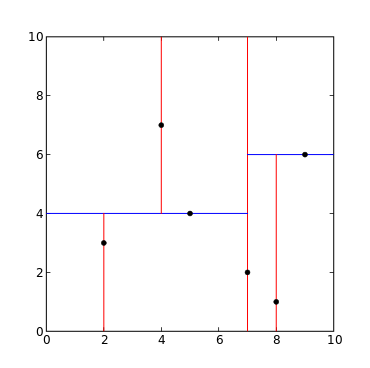
\includegraphics[width=.9\linewidth]{Kdtree_2d.png}
			\caption{An example of a 2d k-d tree\cite{KdTreeFig1}}
		\end{subfigure}%
		\begin{subfigure}{.5\textwidth}
			\centering
			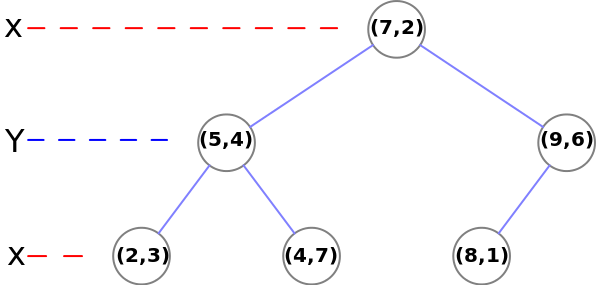
\includegraphics[width=.9\linewidth]{Tree_0001.png}
			\caption{The data structure\cite{KdTreeFig2}}
		\end{subfigure}
		\caption{K-d tree graphic representation}
		\label{fig:kdtree}
	\end{figure}
	
	An implementation of seed selection based on the k-d structure is proposed by Redmond and Heneghan\cite{KdTreeKmeans}. The reason for using this data structure is to gain information about the density of the dataset. In order to suit the problem some decisions have been made while building the tree. At each step the dataset is split among the longest dimension of the bounding box. This box can be computed by taking the minimal and maximal values for each feature in the dataset, and building two new points. The longest dimension is simply the feature for which there is the greatest difference between the two points calculated in the previous step. The chosen condition for stopping and making a leaf node is when the size of the considered dataset is \(\frac{n}{10K}\) or lower, which allows approximatively 10 leaf buckets for each cluster.
	
	After the k-d tree is built some density estimations are made using the obtained leaf buckets. For each bucket the value of the density is calculated as \( N / V \), where N is the number of points it contains and V is the volume of the bounding box. The volume is computed as the product of the differences between each feature of the two bounding points, or the geometric mean in case of two features being equal. 
	
	The heuristic for choosing the seeds is to get points that have a large density and are separated by a reasonable distance. Thus, the first seed is equal to the mean of the bucket with the highest density. The other k-1 seeds are chosen to be the ones that maximize the value g, where g is the product between the density of the bucket mean and the minimum distance to other bucket means. An optimization to avoid outliers is to compute the seeds, remove 20\% of the least dense buckets, and then compute another pair of seeds.
	
	The algorithm was compared to another 3 initialization methods (Forgy, Bradley and Fayyad, Katsavounidis), on 36 datasets and obtained better Distortion values on over 30 compared to each of the other methods. Distortion is the sum of the distances between each point and its cluster center.
	
	\subsubsection{ROBIN}
	ROBIN stands for Robust Initialization and is a method designed by Hasan et al.\cite{ROBIN}, with the main goal to avoid choosing outliers as seeds for the K-means algorithm. For this reason the measure of LOF(Local Outlier Factor) is used. To compute this for a point x, we first need the neighborhood \(N(x, mp)\) on the threshold mp(mininum points). This is a set of all the points closer or equally close to x than the mpth nearest neighbor. The \(density(x, mp)\) value is calculated as the fraction of the size of the neighborhood and the sum of distances between x and all points in N. The average relative density of x, \(ard(x, mp)\), is then computed as the ratio of \(density(x, mp)\) and the average density of its nearest neighbors. The LOF score is then calculated as the inverse of the ard value. 
	
	The algorithm stands from a reference point r, which can be any point in the dataset. It then sorts the points in decreasing order of distances from r and chooses the first point that has a LOF value around 1. In the following iterations, instead of r, the points are sorted in decreasing order of the minimum distances from the points that have been chosen as centers. The worst case computational complexity is \(O(n\cdot logn\cdot k\cdot d)\), due to the sorting method.
	
	The method was evaluated on a set of synthetic datasets, with d(the number of features) varying from 8 to 24 and k going from 10 to 50 and the number of data points generated for each of the clusters being a random value between 100 and 1000. For each of these datasets the ROBIN initialization method has performed better than the random selection method in terms of distortion, and has obtained results close to the optimal ones.
	
	\section{Variants}
	\subsection{Bisecting K-means} 
	bisecting kmeans
	
	\subsection{Evolutionary K-means }
	genetic kmeans
	
	
	\section{Conclusions}
	TODO something conclusive
	
	\newpage
	\bibliography{references_document}
	\bibliographystyle{ieeetr}
\end{document}